\subsection{Methodology}

The main goal in creating the face recognition model was to experiment over the techniques described in \cite{deepface,facenet}.
Specifically, the techniques we will be playing around with are:
\begin{enumerate}
    \item Minimizing the \bf{triplet loss function} \cite[Eq. 1]{facenet} (\href{https://github.com/nicholaspun/IZ-Net/blob/master/faceRecognition/TripletPickerHelper.py}{\inlinecode{TripletPickerHelper.py}}): We use SGD with momentum $0.9$ as suggested in the paper, a batch size of 32, and since there around $\binom{n}{3} \in \bigO(n^3)$ triplets in an $n$-sized training set, we train (very unscientifically) until it takes too long to obtain a batch of semi-hard triplets.
    (The real reason for this was because the Google Collab notebook would become unstable if left on for too long)
    This achieved good enough results according to the tools we'll go over in a bit.

    \item Casting this as a \bf{binary classification} problem \cite[Sec. 4.2]{deepface} (\href{https://github.com/nicholaspun/IZ-Net/blob/master/faceRecognition/PairPickerHelper.py}{\inlinecode{PairPickerHelper.py}}):
    Again, we use SGD with momentum $0.9$ and a batch size of 32.
    For binary classification, since choosing and labelling pairs of images is completely deterministic, we \it{could} train on all $\bigO(n^2)$ samples.
    However, we opted to train only on half the amount of possible samples, again, in the interest of time.
    We note that this many samples was more than sufficient to push the accuracy of the model to be very close to 1 on average.
\end{enumerate}

Both techniques aim to train networks to produce ``\it{suitable}'' image embeddings (feature vectors).
Here, we define suitable to (roughly) mean that the Euclidean distance between embeddings of images from the same members should be minimized, while embeddings of images from different members should be maximized.
To that end, we train 3 different architectures: the ``NN1'' architecture \cite[Table 1]{facenet}, ``NN2'' architecture \cite[Table 2]{facenet} and Keras InceptionNetV3 architecture\footnote{See \url{https://keras.io/api/applications/inceptionv3/}}.

In order to verify our networks, we use 3 different analytical tools (See \href{https://github.com/nicholaspun/IZ-Net/blob/master/faceRecognition/analysis.py}{\inlinecode{analysis.py}})
\begin{enumerate}
    \item \bf{t-distributed Stochastic Neighbor Embedding} (t-SNE) \cite{tSNEPaper}: 
    We use the \it{scikit-learn} implementation\footnote{See \url{https://scikit-learn.org/stable/modules/generated/sklearn.manifold.TSNE.html}} of t-SNE.
    It works fairly well out-of-the-box---the only parameters we modified were the number of iterations (increasing it to 5000) and the perplexity (set to 150).\footnote{I particularly enjoyed reading \href{https://distill.pub/2016/misread-tsne/}{\it{How to Use t-SNE Effectively}} by Wattenberg, Vi\'{e}gas and Johnson as it was quite informative on the consequences of the various parameters}
    These particular values produced sensible results over the range of values we tried out.
    We use t-SNE to quickly determine the degree of clustering of our training set.
    \Cref{Figure:Face-Recognition:method:tsne-example} shows an example of possible outputs of the algorithm and our aim to is produce an plot that looks like \Cref{Figure:Face-Recognition:method:tsne-example:clustered}.
    
    \begin{figure}[htbp]
        \begin{subfigure}[]{0.49\textwidth}
            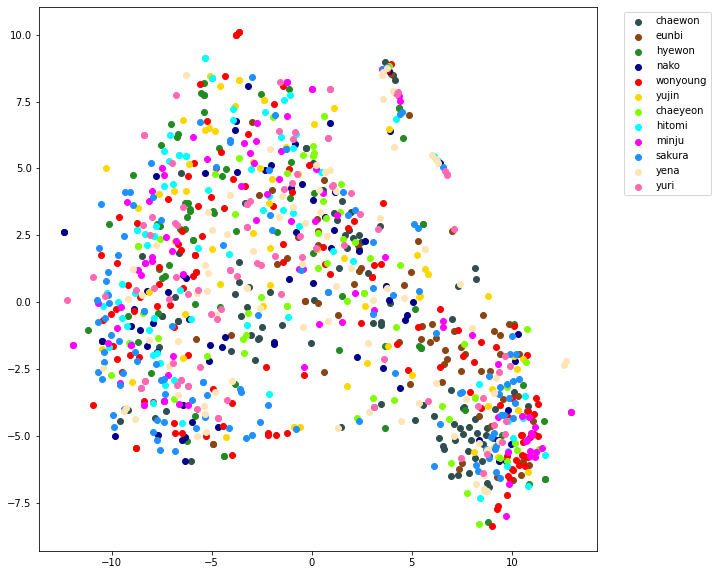
\includegraphics[trim=0 0 100 0, clip, width=\textwidth]{images/faceReco/tsne-example-unclustered.png}
            \caption{Unclustered data}
            \label{Figure:Face-Recognition:method:tsne-example:unclustered}
        \end{subfigure}
        \hfill
        \begin{subfigure}[]{0.49\textwidth}
            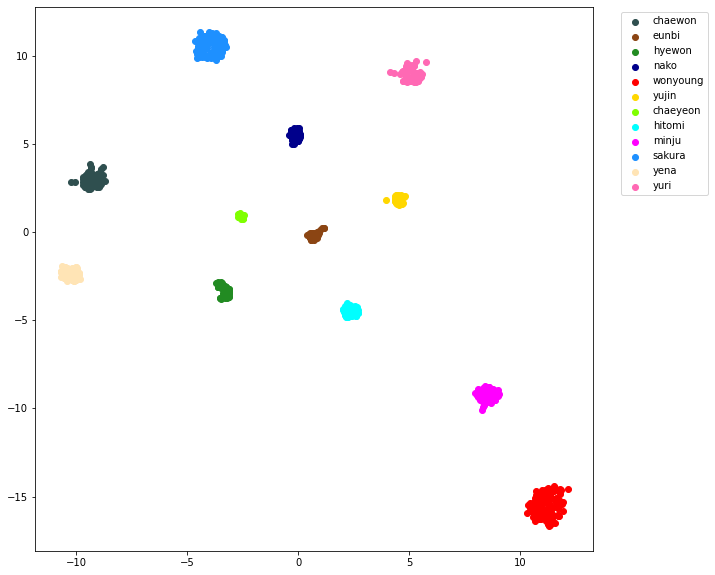
\includegraphics[trim=0 0 100 0, clip, width=\textwidth]{images/faceReco/tsne-example-clustered.png}
            \caption{(Probably) clustered data}
            \label{Figure:Face-Recognition:method:tsne-example:clustered}
        \end{subfigure}
        \hfill

        \caption{Possible outputs of the t-SNE algorithm}
        \label{Figure:Face-Recognition:method:tsne-example}
    \end{figure}

    \item \bf{Boxplot of Pairwise Distances}:
    We compute the pairwise (Euclidean) distances of the image embeddings within the training set for each member and allow \it{matplotlib} to take care of making the boxplot.
    We use this tool to quickly determine the dispersion of image embeddings for each member.
    Ideally we want low dispersion, so we want to see short whiskers and few outliers.
    This tool is also used in conjunction with the next tool.

    \begin{figure}[htbp]
        \centering
        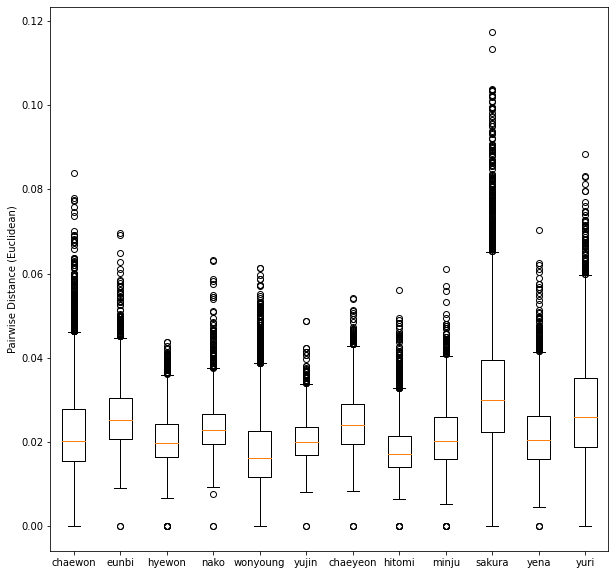
\includegraphics[width=0.68\textwidth]{images/faceReco/boxplot-example.png}
        \caption{An example boxplot of pairwise distances}
        \label{Figure:Face-Recognition:method:boxplot-example}
    \end{figure}
    
    \item \bf{Table of medoid distances}:
    While the boxplot takes care of \it{intra}-member distances, we also need a tool to help us analyze \it{inter}-member distances.
    For each member, we compute the medoid of the image embeddings of their training set and compute the pairwise distances between the medoid for each member.
    This produces a table like \Cref{Table:Face-Recognition:method:medoid-table-example}\footnote{If you're reading this printed, all the tables are in \Cref{Section:Tables-Galore}}.

    To use this along with the previous tool, we note that the distances between the medoids in \Cref{Table:Face-Recognition:method:medoid-table-example} are at least 1.0.
    However, in \Cref{Figure:Face-Recognition:method:boxplot-example}, the distances are all less than 0.12.
    This is an indication that our image embeddings are indeed clustered and there are large distance between clusters. 

\end{enumerate}

Finally, we'll take a brief detour to mention how we obtained our training sets.
While scraping for images is easy, our training set needs to include images of \it{only} the face, as in the 2nd step of \Cref{Figure:Introduction:IZNet-pipeline}.
This is a bit more difficult to come across.
To solve this, we cheat a bit and use a pretrained model along with OpenCV to extract faces out of our images---generating a new dataset consisting only of faces.\footnote{Weights were obtained from the Github link located in the article \href{https://towardsdatascience.com/extracting-faces-using-opencv-face-detection-neural-network-475c5cd0c260}{\it{Extracting faces using OpenCV Face Detection Neural Network}} by Bhanot.}